\documentclass{article}[12pt;letterpaper]
\usepackage{graphicx}
\usepackage{verbatim}
\usepackage{color}
\usepackage[nohead,nofoot,left=1in,right=1in,top=1in,bottom=1in]{geometry}

\pagestyle{empty}
\raggedright
\frenchspacing
\setlength{\parskip}{0in}
\setlength{\parindent}{0in}

\newcommand{\todo}[1]{\textcolor{red}{TODO #1}}

\begin{document}

\begin{flushleft}
Parry Wilcox \\
Andrew Shen
\end{flushleft}

\section{Thread count scaling}

We ran \texttt{nbody -s 1352723313 -nt \$NTHREADS} for \texttt{\$NTHREADS = 1,
2, 4, 8}. For the most part we see the speedup that we expect from using more
threads:

\begin{center}\begin{tabular}{c l}
Thread Count & Time (s) \\
\hline{}
1 & 3.121816 \\
2 & 2.286314 \\
4 & 1.377848 \\
8 & 1.388689
\end{tabular}

% http://chart.apis.google.com/chart?cht=lxy&chs=400x300&chma=16,16,16,16&chxt=x,y&chxr=0,0,8|1,0,3.5,0.5&chds=0,8,0,3.5&chm=D,000000,0,0,2|o,000000,0,,7&chd=t:1,2,4,8|3.121816,2.286314,1.377848,1.388689
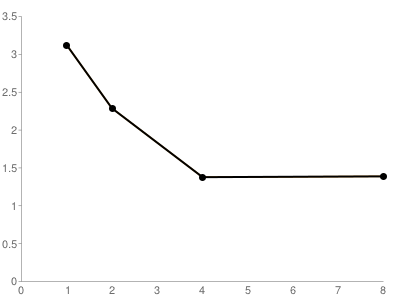
\includegraphics[width=3in]{a2_sec1_1.png}
\end{center}

When we run the same study with irregular particle distribution, we find no
effect on the running times subject to the precision of the timing logic. We
think that this is because the load imbalancer, which prevents the first $1/4$
of particles \textit{in memory} from moving, ends up making the processor
responsible for doing the stopped particles perform \textit{less} work than
the other processors, so that the time is determined by the other processors
due to the use of barriers to enforce sequential operation.

\section{Chunk-scheduled scaling}

We ran \texttt{nbody -b -nt 8 -s 1352723313 -c \$CHUNKS} for \texttt{\$CHUNKS =
1, 2, 4, 8, 16, 32, 64, 128, 256, 512}. We notice that as the chunk size goes
to the number of particles, the load becomes imbalanced because only the first
few threads receive chunks to work on, causing a decrease in performance to a
level comparable to block partitioning with one thread.

\begin{center}\begin{tabular}{c l}
Chunk size & Time (s) \\
\hline{}
  1 & 1.268889 \\
  2 & 1.144190 \\
  4 & 1.185820 \\
  8 & 1.160155 \\
 16 & 1.327447 \\
 32 & 1.249977 \\
 64 & 1.249480 \\
128 & 1.308981 \\
256 & 1.784157 \\
512 & 2.799230
\end{tabular}

% http://chart.apis.google.com/chart?cht=lc&chs=400x300&chma=16,16,16,16&chxt=x,y&chxr=0,0,9|1,0,3&chds=0,3&chm=D,000000,0,0,2|o,000000,0,,7&chxl=0:|1|2|4|8|16|32|64|128|256|512&chd=t:1.268889,1.14419,1.18582,1.160155,1.327447,1.249977,1.249480,1.308981,1.784157,2.79923
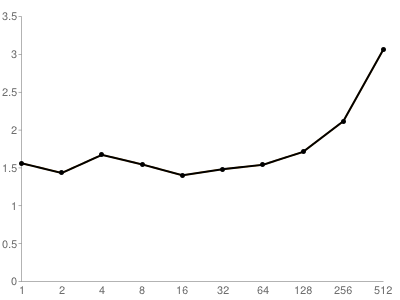
\includegraphics[width=3in]{a2_sec2_1.png}
\end{center}

A similar effect appears without load imbalancing.

\begin{center}\begin{tabular}{c l}
Chunk size & Time (s) \\
\hline{}
   1 & 1.493572 \\
   2 & 1.449901 \\
   4 & 1.285738 \\
   8 & 1.439543 \\
  16 & 1.566758 \\
  32 & 1.327371 \\
  64 & 1.376504 \\
 128 & 1.339076 \\
 256 & 1.838099 \\
 512 & 2.804073 \\
1024 & 4.773173
\end{tabular}

% http://chart.apis.google.com/chart?cht=lc&chs=400x300&chma=16,16,16,16&chxt=x,y&chxr=0,0,10|1,0,5&chds=0,5&chm=D,000000,0,0,2|o,000000,0,,7&chxl=0:|1|2|4|8|16|32|64|128|256|512|1024&chd=t:1.493572,1.449901,1.285738,1.439543,1.566758,1.327371,1.376504,1.339076,1.838099,2.804073,4.773173
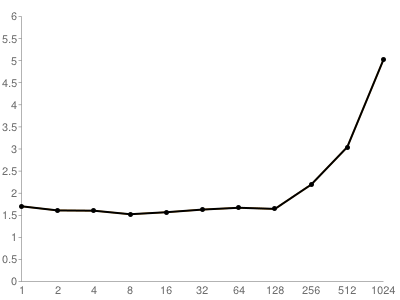
\includegraphics[width=3in]{a2_sec2_2.png}
\end{center}

\section{Comparison of block and chunk partitioning}

We ran block and chunk (size 4) partitioning for each allowed number of threads
(1, 2, 4, 8). There is a comparable speedup between both methods. This is
probably because having the correct chunk size allows dynamic scheduling to
more evenly distribute small blocks of work among workers, so that the speedup
is comparable to the speedup that we get from just throwing more processors at
the problem.

\begin{center}
\begin{tabular}{c l l}
Thread count & Block time (s) & Chunk=4 time (s) \\
\hline{}
1 & 4.153872 & 4.167199 \\
2 & 2.315583 & 2.358403 \\
4 & 1.454456 & 1.433370 \\
8 & 1.437606 & 1.278942
\end{tabular}

% http://chart.googleapis.com/chart?cht=lxy&chs=400x300&chma=16,16,16,16&chxt=x,y&chxr=0,0,8|1,0,4.5&chds=0,8,0,4.5,0,8,0,4.5&chm=o,000000,0,,7|o,000000,1,,7&chls=2|2,5,5&chco=000000&chd=t:1,2,4,8|4.153872,2.315583,1.454456,1.437606|1,2,4,8|4.167199,2.358403,1.433370,1.278942
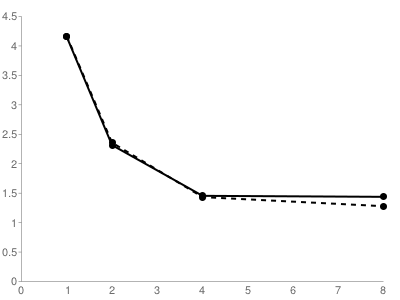
\includegraphics[width=3in]{a2_sec3_1.png}
\end{center}

Dotted line represents chunk partitioning with chunk size of 4.

\section{Performance bottlenecks}

We notice that a lot of time is spent idling at barriers in each thread. This
is probably a consequence of the extremely conservative way in which we
implemented coherence, which needed barriers after every parallel computation
and after every reset of the counter that we used for dynamic chunk scheduling.

We also had problems with data races. \todo{Parry please help me explain this.}

\end{document}
